% !TEX root = 99_main.tex

Please note from this section onward we define "user" or "participant" as occupants and visitors to the new NZEB who used the SDE Learning Trail application, "research team" as our team coordinating the experiment, and "building" as the new NZEB. 

A total of 35 stations (6 trails) were spread across the 6 floors of the new NZEB. The placement of a trail in the building was based on where the building feature was most pronounced. For example, the water trail stations were placed right next to the storm water feature, bio-retention basins and the detention tank for the building. This helped instantly contextualize the digital content of trail and its stations with their physical location in the building.\\

Stations were placed in proximity of fixed sensors measuring 7 attributes in real-time: temperature, humidity, noise, light, carbon-dioxide, volatile organic compounds and presence. The stations were distributed across outdoor and indoor spaces based on trail configuration, station content, proximity to fixed sensors.\\

The interactive mobile web application was launched on Jan 30th, 2019 at the opening ceremony of the new NZEB. Over the next three months - staff \& students from the university, external governmental, industrial and academic delegations were organized into groups for taking guided tours of the new NZEB by the research team with help from NZEB management.\\

Each participant in the guided tours' used the mobile web application to go through trails, scanning stations with the help of an embedded QR code scanner in the application. The application was built in a way such that each user was prompted randomly to provide temperature, light and noise levels feedback 5 times out of all stations visited during the guided tour. A total of 616 users used the application over 3 months, providing 1163 environmental comfort feedback points.\\

The data from the users and fixed sensors was aggregated using a Influx cloud time-series database - which served as a platform for data acquisition, storage and error detection. The combination of location based user comfort feedback and fixed environmental sensor data allowed clustering analysis of personalized comfort profiles of users ,and environmental profiles of spaces. Details regarding outcomes of this period are presented in the results section of this paper. An overview of the experiment setup is provided in Figure\ref{fig:experiments}.\\



\begin{figure}
\begin{center}
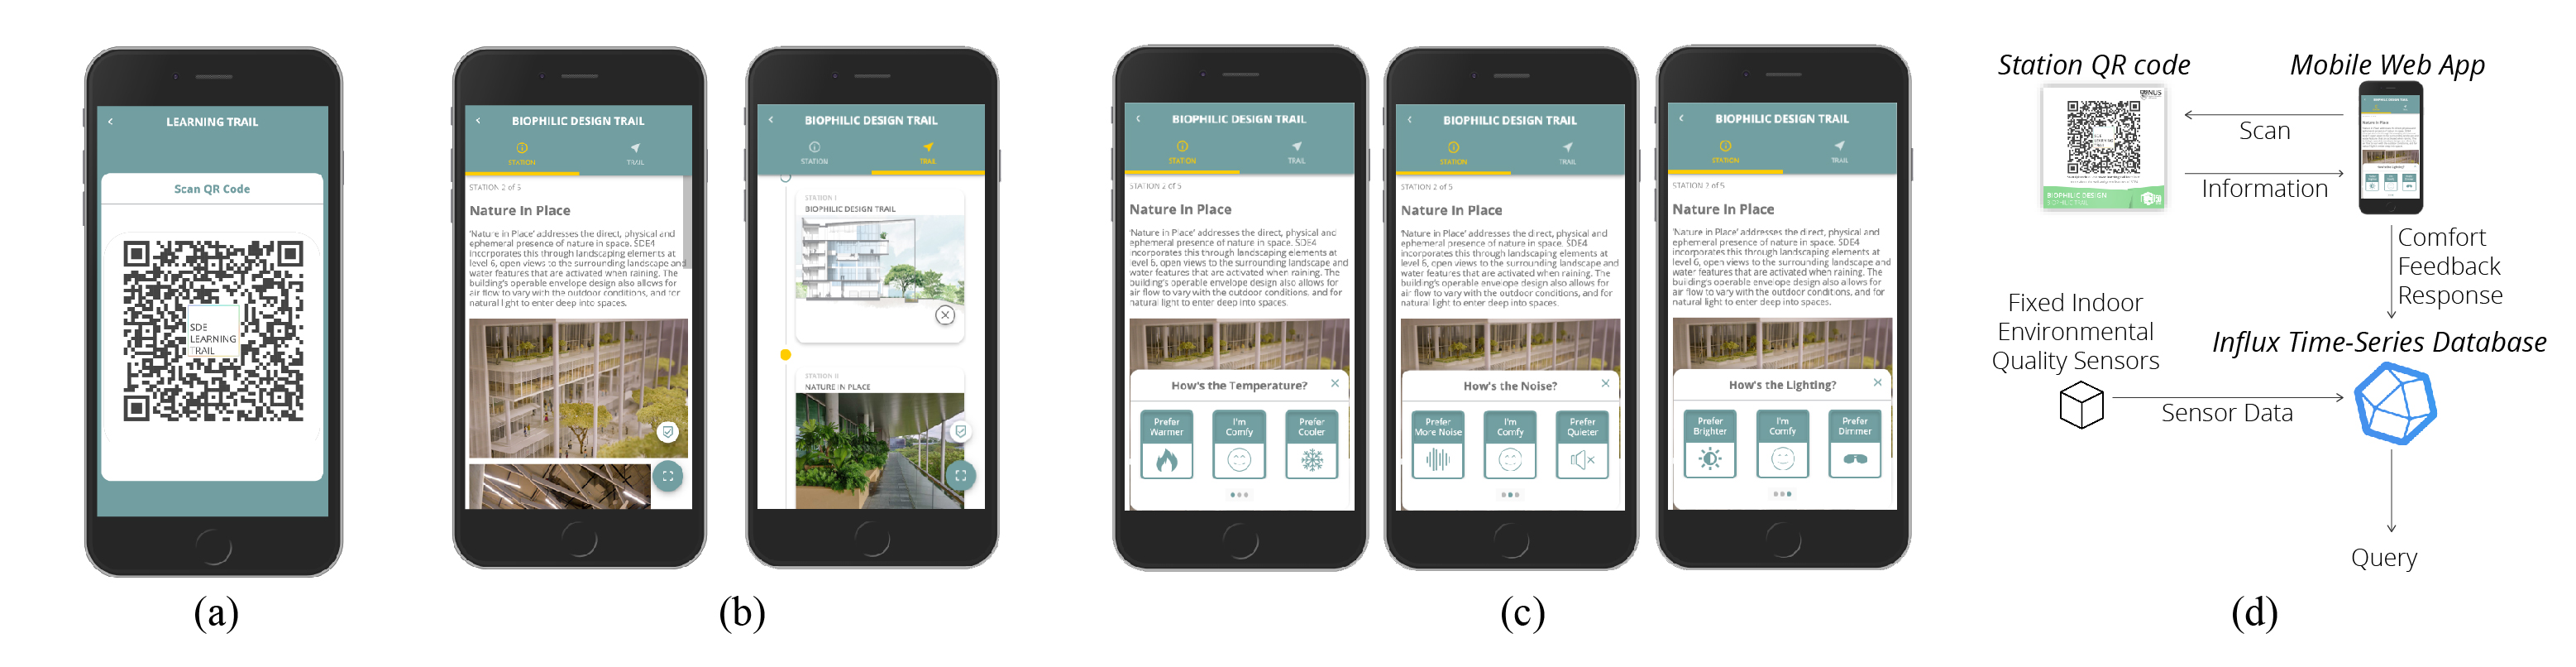
\includegraphics[width=\textwidth, trim= 0cm 0cm 0cm 0cm,clip]{Fig2.jpg}
\caption{Overview of Experiment Setup. (a) Biophilic Design trail as an example of trail placement in the building, (b) Photos from guided tours for participants, (c) Feedback prompts in the application, (d) Overview of data communication.}
\label{fig:experiments}
\end{center}
\end{figure}

